\section{Proposed Protocols}
In this section, we propose transmission protocols that combine the advantages of the previously discussed quantizer and its modification for distributed gradient compression. We first introduce an `All-Out' protocol that fully utilizes the benefits of distributed source coding. Then, we propose a `worker-side' protocol that doesn't utilize the side information from other workers at the encoder side and relies solely on the worker's own gradient. Finally, we introduce a `hybrid' protocol that switches between the `All-Out' protocol and a worker-side protocol to mitigate the accumulation of reconstruction errors over many rounds of training.

Before discussing the protocols, we offer a diagram of the overall encoding and decoding process, which is the same for all protocols, but the side information and the training method of the quantizer changes. Figure~\ref{fig:wz-pipeline} shows this process.

\begin{figure}[htbp]
    \centering
    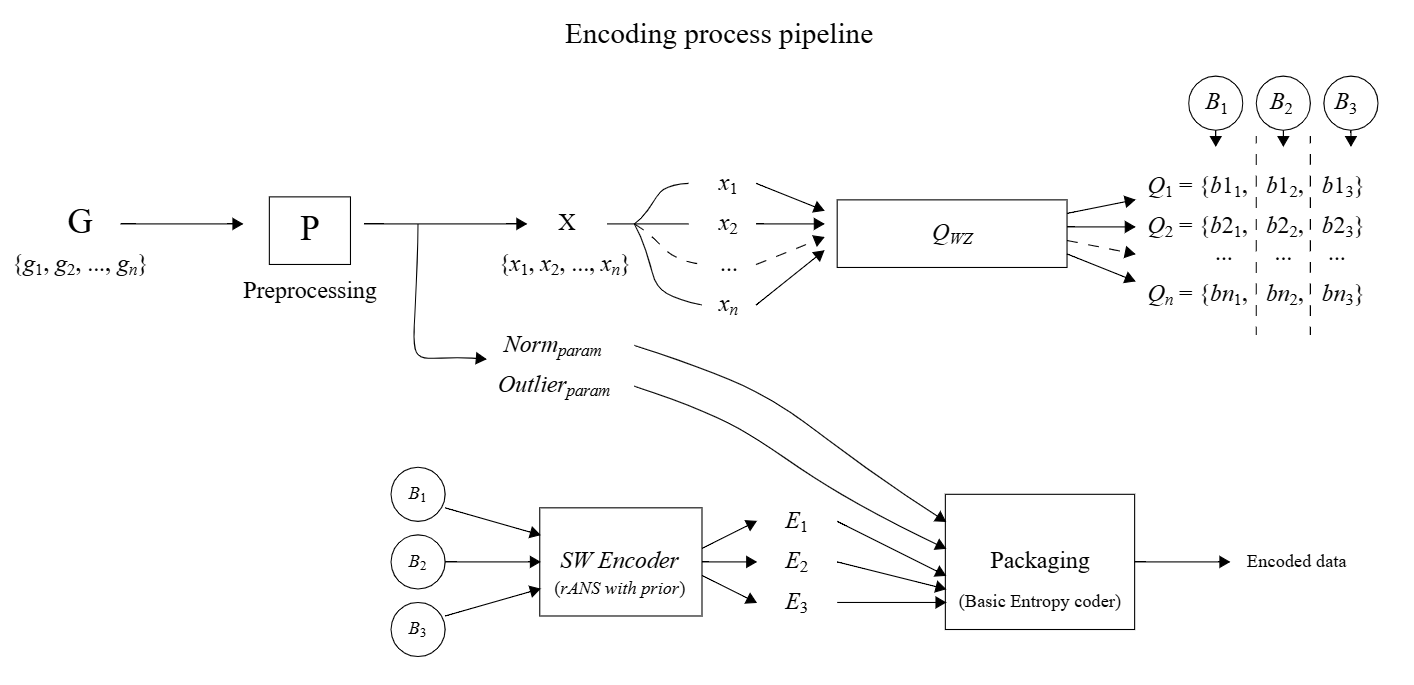
\includegraphics[width=1\textwidth]{Chapters/chapter_3_materials_methods/figures/encoding process}
    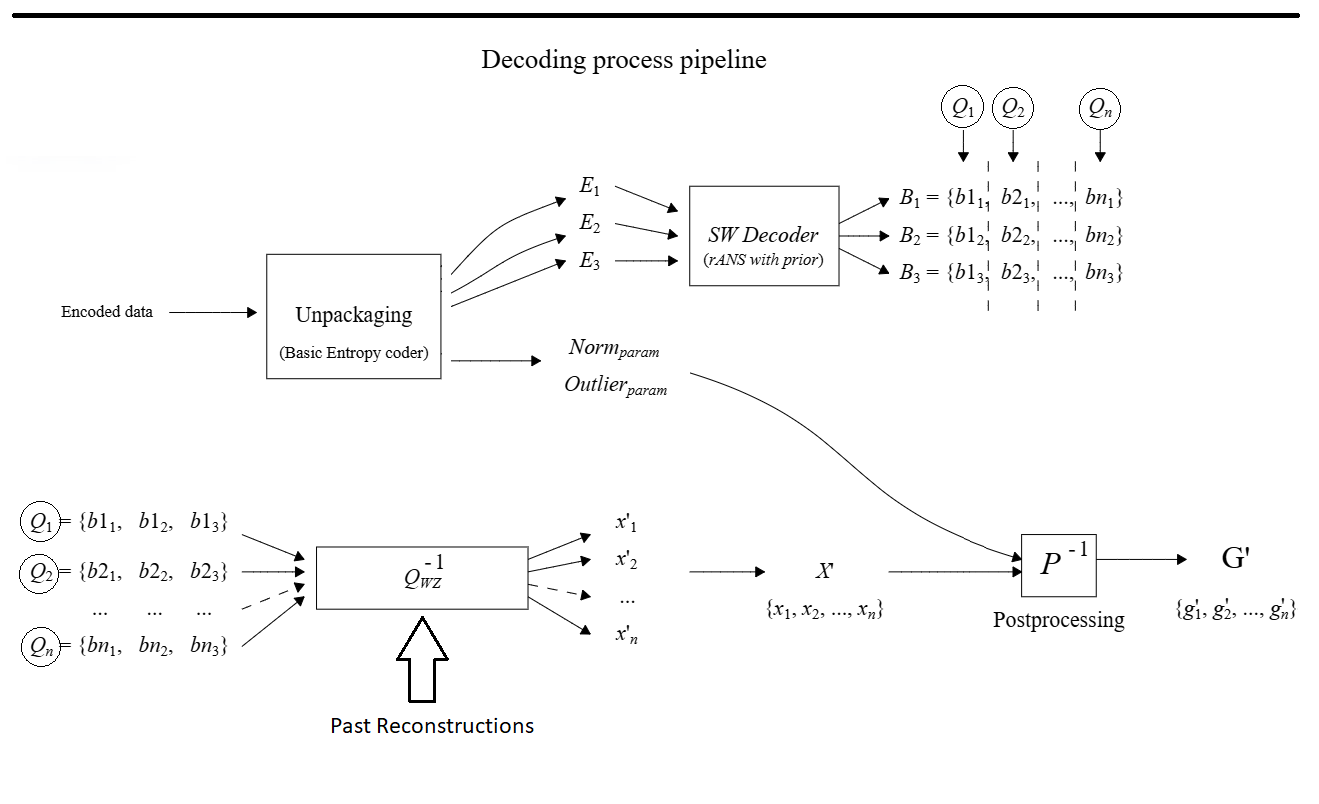
\includegraphics[width=1\textwidth]{Chapters/chapter_3_materials_methods/figures/decoding process}
    \caption{The encoding and decoding process for the proposed protocols. G and G' are the original and reconstructed gradients, respectively.}
    \label{fig:wz-pipeline}
\end{figure}

\subsection{Simple protocol}
As a baseline, we include a barebones protocol that only trains a DSC quantizer once and reuses it for all rounds of communication. For this, the server first sends a non-DSC quantizer to all workers for a warmup phase. This quantizer is discussed more in the next protocol section. After the warmup phase, the server trains a DSC quantizer on the reconstructions of the previous round, using all other workers' reconstructions as side information. The encoder for this quantizer is then sent to all workers, who use it to encode their gradients for the rest of the training. The server uses the decoder to reconstruct the gradients using the side information from all other workers. We also do not use the DSC entropy coder in this protocol, and only use gzip to compress the encoded bin indices, as we assume the prior will not be very accurate after many rounds of training, and the realized rate will be much closer to the marginal rate. Figure~\ref{fig:simple_protocol_performance} shows the performance of this protocol compared to a raw entropy coder (gzip) scheme.

\begin{figure}[htbp]
    \centering
    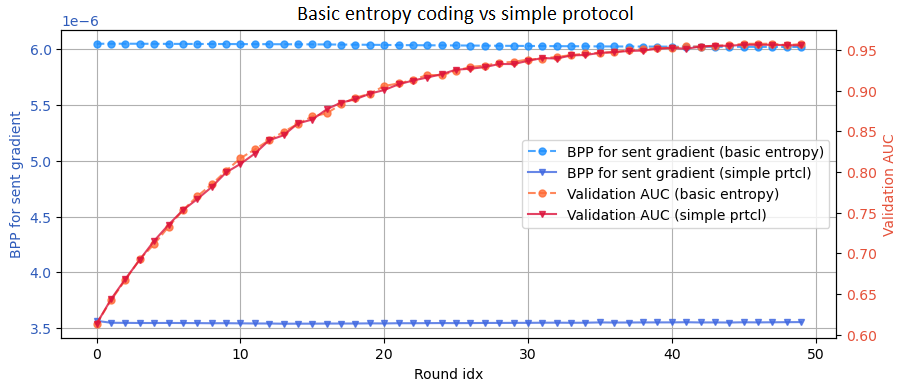
\includegraphics[width=1\textwidth]{Chapters/chapter_3_materials_methods/figures/base_vs_simple}
    \caption{Performance of the simple protocol compared to a raw entropy coder (gzip) scheme. The results are from training a ResNet-18 model on the SVHN dataset with 5 workers. BPP stands for bits per parameter.}
    \label{fig:simple_protocol_performance}
\end{figure}

\subsection{All-Out Protocol}
This is our main proposed protocol that fully utilizes the benefits of distributed source coding by leveraging the side information from all other workers at the encoder side.
In this protocol, the server first sends a non-DSC quantizer to all workers. The first round counts as warmup and will provide us with our first batch of side information which will be used in the next round.
For all subsequent rounds, the server will train a DSC quantizer encoder-decoder pair based on the reconstructions of the previous rounds. The training target will be the last, most recent reconstruction of the worker which will transmit the gradient, and the side information will be all the remaining reconstructions, including from other workers. Also, as the number of side information increases, we can use a lower bit rate for the quantizer to achieve lower communication cost without sacrificing much performance. We always use 2 stages for the quantizer, but the number of bins starts from 16 and goes down to 4 as the number of side information increases. Below you can see the exact equation we used:
\begin{equation}
    \text{num\_bins} = \max\left(\left\lfloor\frac{16}{\left(\frac{\text{curr\_round\_idx}}{2}+1\right)}\right\rfloor, 4\right)
\end{equation}

Then the server will only send the encoder to the worker in question which will be used to encode the gradients at the worker side. This encoder tends to be very small in size, constantly below 100 KB, so the communication cost of sending the encoder is negligible compared to the cost of sending the model weights from server to worker, and also the gradients from the worker to server. The decoder will be kept at the server side and will be used to reconstruct the gradients using the side information from all other workers.
In a synchronous Federated Learning setting, we will have exactly $k \times n - 1$ side information available when training the quantizer, where $k$ is the number of workers and $n$ is the number of previous rounds we want to use as side information, and the $-1$ is because we don't use the worker's own reconstruction as side information, but only as the target. At this point, the model should have an encoder which only takes the gradients, and a decoder which takes the encoded gradients as bin indices, and all the side information it had during training.
The server will send the quantizer to the worker in question and the worker will encode its gradient to get a list of bin indices alongside some parameters relating to normalization and outlier handling. Now this list of bin indices should be encoded further using a lossless DSC entropy coder. Due to complexity, this step is simulated in our experiments, as we'll discuss in the later section 3.6. The final package is given to a normal compressor like gzip to remove any remaining redundancy, especially regarding the normalization and outlier parameters.
At the decoder side, the server will first decode the package using gzip and the DSC entropy decoder. Then, the server will use the quantizer's decoder to reconstruct the gradient using the decoded bin indices and all the side information it has from other workers. The schematic in Figure~\ref{fig:all_out_protocol} shows the overall transmission protocol.

\begin{figure}[htbp]
    \centering
    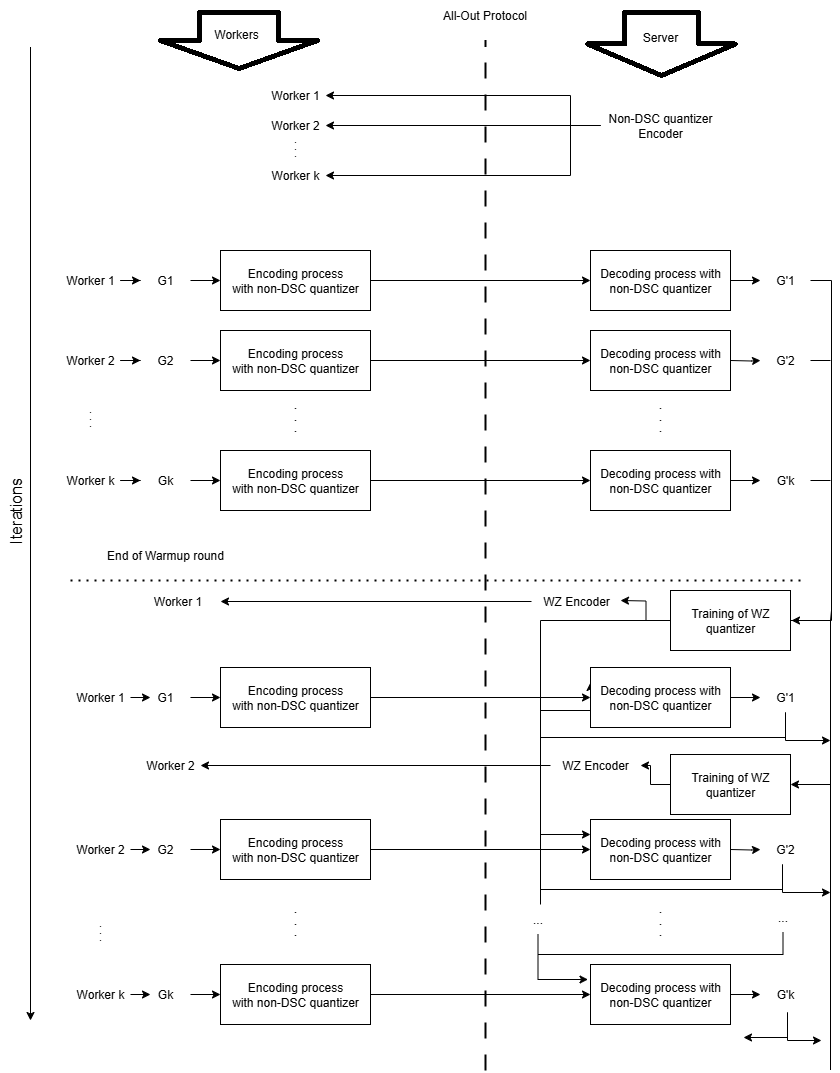
\includegraphics[width=1\textwidth]{Chapters/chapter_3_materials_methods/figures/all-out-protocol.png}
    \caption{Schematic of the `All-Out' protocol. The server sends a non-DSC quantizer to all workers at the start of training. In the next rounds, the server sends a DSC quantizer trained on the reconstructions of the previous rounds. This way, the quantizer can utilize the side information from all other workers to improve its performance.}
    \label{fig:all_out_protocol}
\end{figure}

Figures~\ref{fig:all_out_protocol_performance} and~\ref{fig:all_out_protocol_mape} show the performance of this protocol compared to the simple protocol in terms of MAPE, training accuracy, and communication cost in bits per parameter (bpp). As we can see, the `All-Out' protocol significantly outperforms the simple protocol in terms of communication cost, but has a slightly higher MAPE, possibly due to the accumulation of reconstruction errors over many rounds of training.

\begin{figure}[htbp]
    \centering
    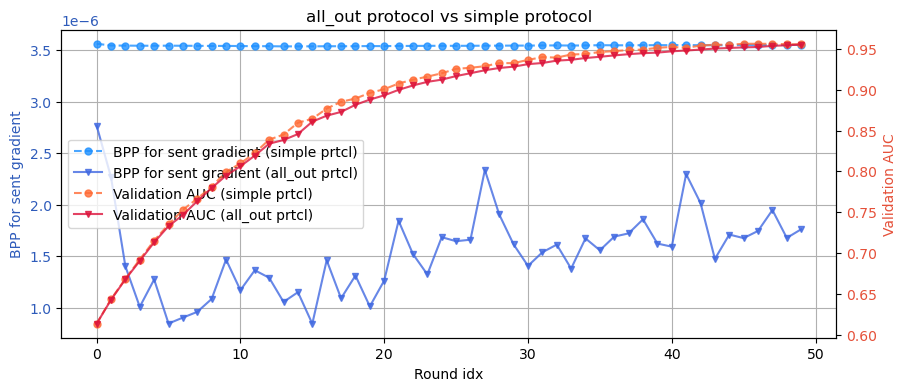
\includegraphics[width=1\textwidth]{Chapters/chapter_3_materials_methods/figures/simple vs all out.png}
    \caption{Performance of the `All-Out' protocol relative to the simple protocol}
    \label{fig:all_out_protocol_performance}
\end{figure}

\begin{figure}[htbp]
    \centering
    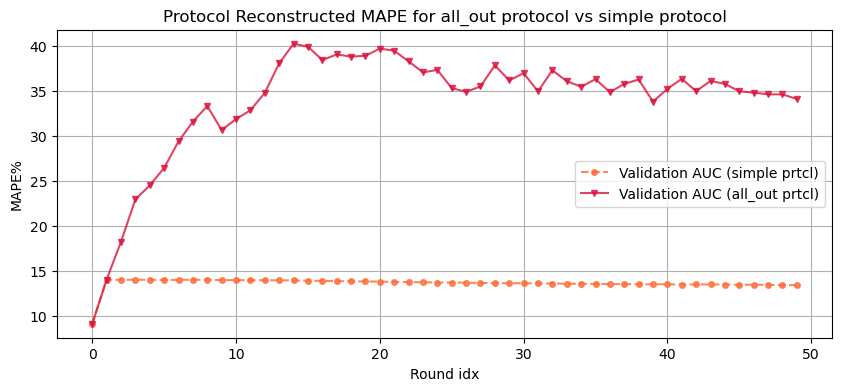
\includegraphics[width=1\textwidth]{Chapters/chapter_3_materials_methods/figures/simple vs all out - mape.png}
    \caption{MAPE values for the same experiment.}
    \label{fig:all_out_protocol_mape}
\end{figure}

\subsubsection{Notes regarding non-DSC quantizer used during warmup}
This quantizer should have a high rate due to 2 related issues:
\begin{enumerate}
    \item Lower rate means fewer bins, which means the reconstruction will be centered on only a few values. This will force the next quantizer that's trained on these reconstructions to also have its bins centered around these values. This will essentially limit the future quantizers to only have as many bin regions (not bins, but the separation regions) as the first quantizer.
    \item The second issue is related to the first, but is more related to accumulated distortions. If the first quantizer has a high distortion, the next quantizer will be trained on these distorted reconstructions, and will learn to reconstruct these distorted values. Over time these distortions will accumulate and the reconstructions will drift away. We discuss this more in the subsection about the hybrid protocols.
\end{enumerate}

\subsubsection{Fingerprinting effect and realized bit-rate}
This part discusses issues with feeding the quantizer model more side information that's not greatly related, for example in a non-IID Federated Learning scenario where the correlations are lower (\cite{ZhangTao2022}, \cite{zhang2024tacklingnoniid}). Due to the fact that the prior is a trained model, having less related side information might cause the prior to overfit, especially when the number of training samples are smaller or the bit rate is smaller. We call this effect fingerprinting, as the prior model will learn a fingerprint for each input value based on the side information. This could be a good thing in a protocol like the `Worker-Side' protocol which will be discussed later.

Regarding the `All-Out' protocol, a lot of assumptions have to be made about how this model will behave when it's trained on the reconstructions of past gradients for both side info and target, and is then used to encode a new, unseen gradient for the next round. This causes the realized rate to be different from the rate given by the prior model in the quantizer. This discrepancy is expected and normal; after all, the model is working on unseen data, and the prior is only an estimate of the training data. (See section 3.6 for information regarding realized and prior rate.) For the 50th round of training ResNet-18 on SVHN with 5 workers, this discrepancy reaches 30\% while the distortion is 2000\% more. This is a big difference, but it is unavoidable with this protocol simply because we work with unseen gradients.

There is a breaking point to this though; assume we have not that many combinations of input and side information, but have a huge number of side information per sample of input, and/or we have a very low bin allocation. Since the prior is a learned model itself, it might start memorizing the side information; in a way it will learn a fingerprint for each input value based on the side information. This could be a good thing in a protocol like the `Worker-Side' protocol, where the input is pre-determined and expected. The quantizer is essentially encoding the positions of the gradients in its own parameter based on the side information. But for the `All-Out' protocol, this might cause issues. If the gradient vector is not that big (small global model), and we use too many side information, the quantizer might start to learn a fingerprint for each input value based on the side information, and in a way overfit to the training data, lowering the rate, and even increasing the distortion.

Now the important takeaway from this section is that we are probably not seeing this effect to be too strong in our experiments. We are using a ResNet-18 model which has around 11 million parameters, and we are using 5 workers, which at most have access to $k \times n - 1 = 5 \times 25 - 1 = 124$ side information per sample. And we are using a bin allocation of a minimum of 6 bins per our 2-stage quantizer, so we can't make a fingerprint for any large portion of the 11 million input values. So we probably are not in the regime where this effect is too strong. But it is something to consider when using this protocol on smaller models, or with more workers, i.e., side information, or with lower bin allocation.

\subsection{Worker-Side Protocol}
This protocol is meant as one of the baselines to compare the improvements gained from using other workers' side information. Hence some might not consider it as much of a DSC protocol, even though it fits the definition, mostly because we are leveraging the temporal correlation of the same worker's gradients, and not the correlation between different sources like other workers. But it offers some advantages as the model will have access to the reconstructions of its own gradients, which will also be available at the server side. This way, the model can be trained to behave exactly the same at both the worker and server side. Compare this with the `All-Out' protocol, and consider the discussion regarding fingerprinting effects in the previous section.
In this protocol, similar to the `All-Out' protocol, the server sends both a non-DSC quantizer for the warmup phase, but this time it's both the encoder and decoder pairs. The aim is to allow the workers to have access to the reconstructions of their own gradients which will be used for training their future DSC quantizers. This model could also be trained at the worker side, but as discussed, the quantizer models tend to be very small in size and it's not an important choice.
For the coming rounds which will be using DSC, instead of training our DSC quantizer at the server, using all reconstructions from all workers, we switch to a worker-side training, hence the name. The training target and side information will be restricted by the available information at the workers. At each worker, we know its gradient, and after training an encoder-decoder pair on that gradient, it can also know the reconstruction of said gradient. We also know that the server will be using the same decoder so the worker and server would know the same reconstructions at all times. This allows us to use the worker's own past reconstructions as side information, and the exact gradient as the target. This way, we minimize the distortion between the original gradient and the reconstruction at both the worker and server side.
The benefit of this protocol might not be obvious, as it only leverages the temporal correlation of the same worker's gradients. Naively, one might think this approach is less desirable as we are not using other workers' correlation which could reduce the rate, and which is the main focus of this thesis. But we must consider that the rate reduction is only as valuable as the reconstruction quality. And one could argue by training the model on the exact gradients, we are getting a lower rate per distortion. Unfortunately we could not get the exact answer due to time limitations. Multiple models, with decreasing bins per stage would have to be trained for both protocols, and then compared, which is very time consuming. So instead we only compare one configuration with a lower bin allocation. The quantizers will have 2 stages, and the bins per stage will follow the equation below which starts at 8 instead of 16, and goes down to 2 instead of 4 in the `All-Out' protocol. On top of that, in this protocol, the fingerprinting effect would become an asset and reduce the rate even more. So we expect this protocol to have a lower rate per distortion compared to the `All-Out' protocol, even with less side information.
As an extra, this protocol has the prior available at both the worker and server side, so we don't need to develop a DSC entropy coder to get the conditional rate, and the rANS could be used as is.

\begin{equation}
    \text{num\_bins} = \max\left(\left\lfloor
\frac{8}{\left(\frac{\text{curr\_round\_idx}}{2}+1\right)}\right\rfloor, 2\right)
\end{equation}

Figure~\ref{fig:worker_side_protocol_performance} shows the performance of this protocol in terms of MSPE, training accuracy, and communication cost in bits per parameter (bpp) compared to the `All-Out' protocol. As we can see, this protocol outperforms the `All-Out' protocol in terms of communication cost and MSPE, which supports our hypothesis regarding the benefits of training the model at the worker side.

\begin{figure}[htbp]
    \centering
    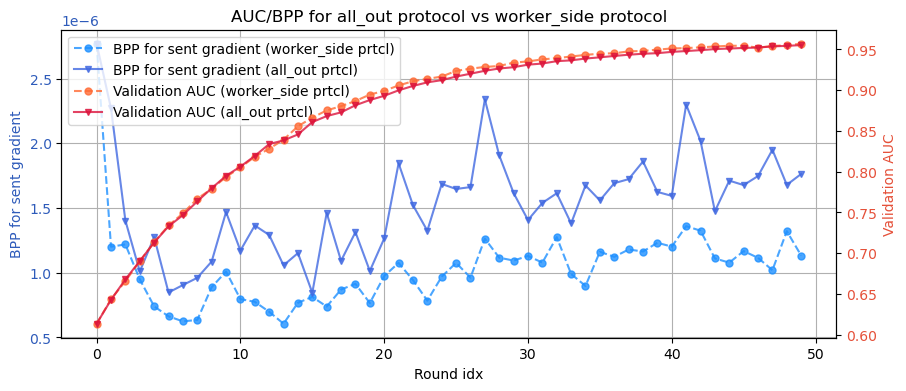
\includegraphics[width=1\textwidth]{Chapters/chapter_3_materials_methods/figures/worker-side vs all out.png}
    \caption{Performance of the `Worker-Side' protocol compared to the `All-Out' protocol.}
    \label{fig:worker_side_protocol_performance}
\end{figure}

\subsubsection{Worker-Side Protocol with Accumulated Error}
This protocol is a modification of the `Worker-Side' protocol, where instead of training on gradients and sending the encoded gradients, we also include the accumulated error from previous rounds. This is similar to the error feedback mechanism used in some gradient compression methods~\cite{Seide}. The idea is to keep track of the error between the original gradient and the reconstructed gradient, and add this error to the next gradient before encoding it. This way, we can reduce the distortion caused by the quantization and improve the overall performance. This goes further in supporting the benefits of training the model at the worker side.

\subsection{Hybrid Interval Switching Protocol}
An issue that arises during many rounds of training, especially at lower bit rates with more side information, is the accumulation of reconstruction errors.
This is because in the `All-Out' protocol, the model is trained on the reconstruction of the previous round, not the original gradient which is at the decoder. The model is essentially using past reconstructions as side information, and learns to reconstruct the most recent reconstruction from the last round. This will slowly lead to a drift away from the original gradient, but more importantly, it would cause an increase in the rate.
To improve the performance of the `All-Out' protocol, we propose a hybrid protocol that switches from the `All-Out' protocol to a `Worker-side' protocol for some time after every $K$ rounds of training and then switches back to the `All-Out' protocol. This way, the model is occasionally trained on the original gradient at the cost of increased communication cost. The switching interval and the duration of the `Worker-side' protocol depends on how well the `Worker-side' protocol performs compared to the `All-Out' protocol. If the gradients depend more on their own temporal changes rather than gradients of other workers, the switching interval can be shorter and the duration of the `Worker-side' protocol can be longer.

In Figure~\ref{fig:hybrid_protocol}, we see that the hybrid protocol keeps the reconstruction error (MSPE) low for many rounds after switching back to the `All-Out' protocol.

\begin{figure}[htbp]
    \centering
    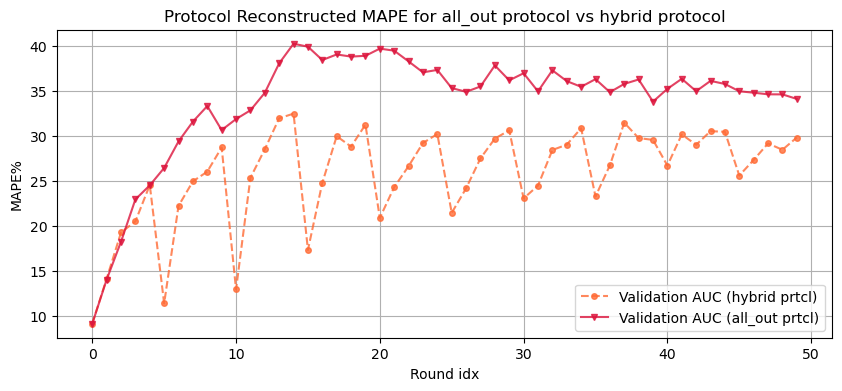
\includegraphics[width=1\textwidth]{Chapters/chapter_3_materials_methods/figures/hybrid vs all out - mape.png}
    \caption{The effect of the hybrid protocol on the reconstruction error (MSPE) over the training rounds}
    \label{fig:hybrid_protocol}
\end{figure}

\subsubsection{Effect of High Reconstruction Error on Training Performance}
This opens up a separate discussion about how much distortion can be tolerated in the gradient without affecting the training performance. We have seen that even with a high MSPE, the training performance can be good. But in our experiments, we noticed that if the MSPE goes above a certain threshold, around 400\%, the training performance starts to degrade. And after enough rounds of the `All-Out' protocol, the training starts to diverge completely.
